% ============================================================================
% Evaluación en el Unitree G1 simulado (MuJoCo). Generada con pabe_cbf.g1.*
% Figuras en figures/, tablas en tables/. Requiere graphicx, booktabs, enumitem.
% ============================================================================
\section{Evaluación en el Unitree G1 simulado}
\label{sec:g1}

\subsection{Plataforma}
\label{sec:g1:platform}
Para someter la propuesta a una prueba más exigente que la abstracción planar se construyó
un banco en MuJoCo~3.16 con el modelo oficial del Unitree~G1 con manos diestras (MuJoCo
Menagerie). Su configuración es la siguiente:
\begin{itemize}
\item \textbf{Robot y control.} La base del robot se fija, porque la propuesta asume un controlador de cuerpo completo que
estabiliza la locomoción, y se estudia el brazo derecho (7~GDL). El brazo se controla por par
calculado con los límites de par del G1 (25\,N\,m en hombro y codo, 5\,N\,m en la muñeca). La física corre a 500\,Hz,
el filtro CBF a 100\,Hz y el HMM a 33\,Hz. El comando articular está limitado en velocidad (2{,}5\,rad/s) y en
aceleración (50\,rad/s$^2$), igual para todos los métodos, incluido B0.
\item \textbf{Geometría y humano.} Los eslabones se aproximan con cápsulas de seguridad
(brazo, antebrazo y muñeca) y la palma con una esfera. La distancia y su gradiente se obtienen de forma exacta
con la distancia segmento--segmento y los jacobianos de MuJoCo. El humano es cinemático en 3D (torso,
cabeza, brazo, antebrazo y mano), con IK de dos eslabones. El agarre se modela como un resorte
físico ($K=300$\,N/m) aplicado a la palma del robot.
\item \textbf{Percepción.} La percepción visual llega con 33\,ms de retardo, que se
incorpora a la cota de error mediante el conjunto alcanzable.
\item \textbf{Robustez.} La perturbación de actuación $w$ de la Ec.~\eqref{eq:dyn} se identifica en
entrenamiento como el percentil 99{,}9 del error de velocidad cartesiana de los puntos de control,
$w=0{,}176$\,m/s. La familia de perturbación, que viola A2 a propósito, queda excluida de esta identificación.
\end{itemize}

Las nueve familias de escenarios amplían las seis de la Sec.~\ref{sec:benchmark} con tres más:
(vii)~embestida breve de la mano humana hacia el antebrazo del robot, que provoca pérdida temporal de
factibilidad; (viii)~retirada ambigua, con señales débiles y lentas, alta entropía y retirada real; y (ix)~humano
\emph{reactivo}, que se retira si el robot invade su espacio sin autorización, se acerca deprisa o tira
con fuerza. Este último cierra el lazo humano--robot.

\subsection{Protocolo y garantías de equidad}
\label{sec:g1:fair}
\begin{enumerate}[label=(\roman*)]
\item \textbf{Un único núcleo de decisión.} Todos los métodos (B0--B9, A1--A11) ejecutan las mismas
funciones de señales de riesgo y del QP (\texttt{pabe\_cbf/core.py}). Un método se distingue sólo por los
campos de su especificación. Comparten el nominal, la geometría, las restricciones físicas, los permisos de
contacto, la política de respaldo, los límites de actuación y las semillas.
\item \textbf{Parámetros elegidos en validación y no en test.} Cada método con umbral de liberación (B3,
B4, B5, B8, B9, A6, A8, A11) usa el de menor cancelación falsa entre los que detectan al menos el
80\,\% de las retiradas en $\le$1\,s, sobre participantes de validación (3000+). B3 y B5 no alcanzan
esa sensibilidad y operan en su punto de máxima sensibilidad. El nivel $\alpha$ de B5 (CRC) se elige junto con su umbral.
La ley exógena de B6 se elige barriendo $\kappa\in\{1,2,4,8,16,\infty\}$ (B6$^\ast$: mínima
infactibilidad y, a igualdad, menor jerk). Los valores elegidos fueron
$\tau_{\rm B9}=0{,}85$, $\kappa^\ast=1$ y $\alpha_{\rm B5}=0{,}4$.
\item \textbf{Adaptaciones corregidas antes de evaluar.} Al inspeccionar el comportamiento se detectaron
y corrigieron tres defectos que penalizaban a comparadores concretos, no a B9:
\begin{itemize}
\item B4 y B5 nunca podían entrar en contacto, porque la entrada segura se comprobaba con su margen de aproximación.
Ahora se comprueba con el margen del modo destino.
\item B5 usaba un cuantil sin contexto. Ahora se condiciona a la velocidad de la mano.
\item En el agarre, el par muñeca--mano humana recibía margen social. Ese margen se anuló para todos los métodos.
\end{itemize}
Tras las correcciones, todos los métodos completan apretones estables.
\item \textbf{Particiones disjuntas por participante.} Entrenamiento (12), calibración (10), validación (6)
y test (20 participantes $\times$ 9 familias $\times$ 2 semillas $=360$ episodios por método).
El 25\,\% de validación y test presenta cambio de dominio. La sensibilidad y el experimento controlado
usan participantes distintos (5000+ y 6000+).
\item \textbf{Estadística.} Las tasas llevan IC~95\,\% de Clopper--Pearson. Los contrastes usan bootstrap pareado
remuestreando participantes (4000 réplicas), y la familia de 17 contrastes pre-registrados se corrige con Holm.
\end{enumerate}

\begin{figure*}[!t]
\centering
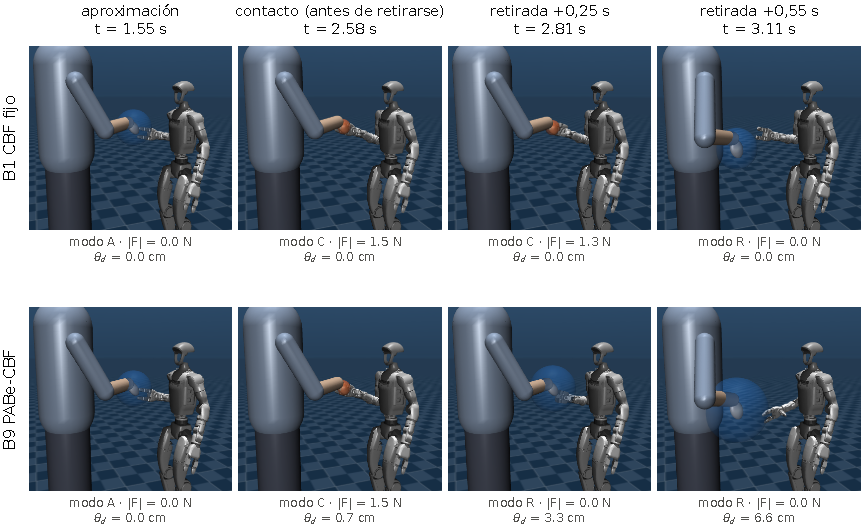
\includegraphics[width=\textwidth]{figures/g1_scene.pdf}
\caption{Retirada durante el contacto en el G1 (MuJoCo). Esfera azul translúcida: margen
$d^{\rm sep}+\epsilon_d+\theta_d$ alrededor de la mano humana fuera del contacto; naranja: agarre activo.
B9 anticipa la retirada con $p_W^+$ y suelta antes. B1 sólo suelta por el tirón táctil explícito y la
fuerza supera $F_{\rm phys}$ (Fig.~\ref{fig:g1ts}d). Vídeo: \texttt{media/g1\_B1\_vs\_B9.mp4} en el repositorio.}
\label{fig:g1scene}
\end{figure*}

\begin{figure*}[!t]
\centering
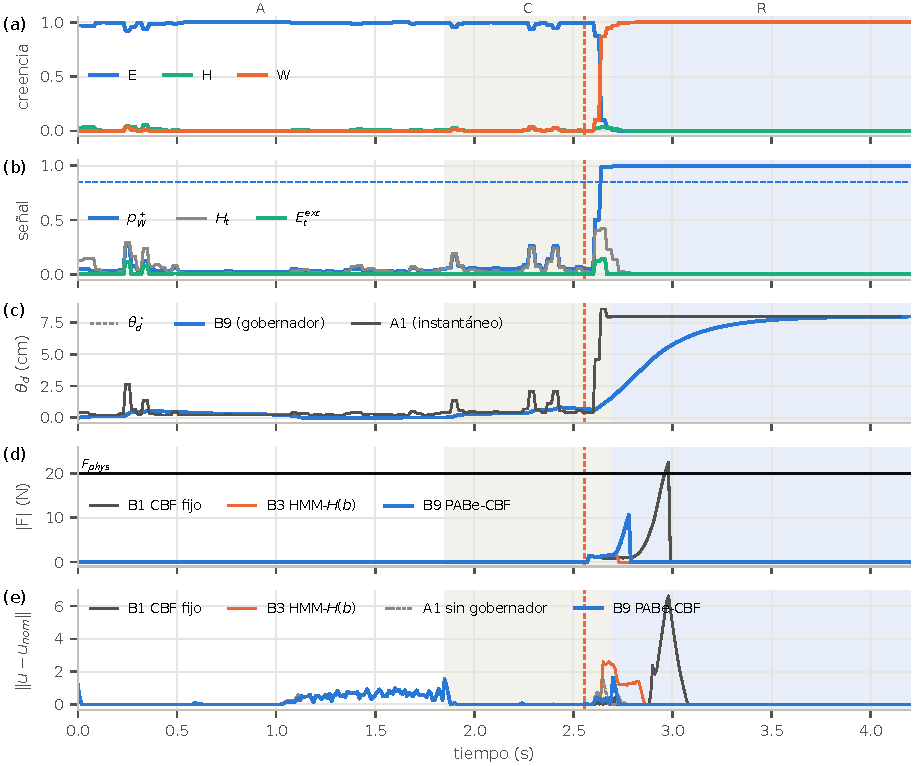
\includegraphics[width=\textwidth]{figures/g1_timeseries.pdf}
\caption{Señales internas del episodio de la Fig.~\ref{fig:g1scene}: (a) creencia; (b) $p_W^+$, $H_t$ y
$E^{\rm exc}_t$ con el umbral $\tau$; (c) margen $\theta_d$ integrado por el gobernador frente al salto instantáneo
de A1; (d) fuerza de interacción; (e) corrección $\|u-u_{\rm nom}\|$. Líneas rojas verticales: ciclos con QP infactible.}
\label{fig:g1ts}
\end{figure*}

\subsection{Resultados globales y por escenario}
\label{sec:g1:main}
La Tabla~\ref{tab:g1main} resume los 20 métodos y la Fig.~\ref{fig:g1scen} los desglosa por escenario.
\begin{itemize}
\item \textbf{Seguridad física.} B9 no registró violaciones en 360 episodios, lo que da una cota unilateral del 0{,}8\,\% bajo el
supuesto i.i.d. Lo mismo ocurre con los métodos con regla semántica de retirada. En cambio, B1 viola el límite de fuerza en el 3{,}6\,\%
de los episodios, SHIELD (B7) en el 18{,}1\,\% y el nominal sin filtro (B0) en el 25{,}6\,\%. En todos los casos la causa son
retiradas durante el contacto (iii) y perturbaciones (vi): con límites de aceleración, el robot no puede seguir un
tirón rápido y la liberación por tirón explícito llega tarde.
\item \textbf{Liberación.} Ninguna liberación de B9 falló, frente al 37\,\% de B1 y el 62\,\% de B7.
\item \textbf{Utilidad.} El coste de la seguridad recae en la utilidad. B9 completa el 64\,\% de los apretones autorizados con un
30\,\% de cancelaciones falsas. Esa tasa la dominan dos familias en las que \emph{ningún} método filtrado evita la pérdida
de factibilidad: la oclusión (v), por la expansión del conjunto alcanzable, y la embestida (vii).
\end{itemize}

\begin{table*}[!t]
\centering\footnotesize
\caption{Resultados en el G1 simulado (MuJoCo), test con participantes no vistos (360 episodios por método, 9 familias). IC 95\,\% Clopper--Pearson.}
\label{tab:g1main}
\setlength{\tabcolsep}{3.2pt}
\resizebox{\linewidth}{!}{%
\begin{tabular}{lrrrrrrrrrr}
\toprule
Método & Viol. \% & Fuerza \% & Eslabón \% & Lib. fallida \% & Sens. \% & Canc. falsa \% & Éxito \% & Infact. \% & Jerk p95 & $J_{int}$ \\
\midrule
B0 nominal & 25{,}6 \scriptsize[21{,}1, 30{,}4] & 25{,}3 & 0{,}0 & 74{,}6 \scriptsize[65{,}9, 82{,}0] & 0{,}0 & 0{,}0 \scriptsize[0{,}0, 1{,}8] & 100{,}0 & 0{,}0 & 160 & 0{,}000 \\
B1 CBF fijo & 3{,}6 \scriptsize[1{,}9, 6{,}1] & 3{,}6 & 0{,}0 & 37{,}1 \scriptsize[21{,}5, 55{,}1] & 0{,}0 & 27{,}8 \scriptsize[21{,}7, 34{,}6] & 69{,}7 & 43{,}9 & 211 & 0{,}204 \\
B2 HMM-MAP & 0{,}0 \scriptsize[0{,}0, 1{,}0] & 0{,}0 & 0{,}0 & 0{,}0 \scriptsize[0{,}0, 16{,}1] & 42{,}4 & 45{,}1 \scriptsize[38{,}0, 52{,}4] & 48{,}7 & 80{,}3 & 242 & 0{,}350 \\
B3 HMM-$H(b)$ ($\tau$=0{,}4) & 0{,}0 \scriptsize[0{,}0, 1{,}0] & 0{,}0 & 0{,}0 & 0{,}0 \scriptsize[0{,}0, 10{,}3] & 41{,}4 & 53{,}9 \scriptsize[46{,}6, 61{,}1] & 45{,}0 & 70{,}0 & 234 & 0{,}192 \\
B4 BCBF ($\tau$=0{,}3) & 0{,}3 \scriptsize[0{,}0, 1{,}5] & 0{,}3 & 0{,}0 & 1{,}4 \scriptsize[0{,}0, 7{,}4] & 78{,}8 & 54{,}1 \scriptsize[46{,}6, 61{,}6] & 45{,}3 & 79{,}4 & 254 & 0{,}238 \\
B5 CRC-CBF ($\tau$=0{,}7) & 0{,}0 \scriptsize[0{,}0, 1{,}0] & 0{,}0 & 0{,}0 & 0{,}0 \scriptsize[0{,}0, 41{,}0] & 71{,}0 & 53{,}5 \scriptsize[46{,}3, 60{,}6] & 42{,}4 & 66{,}7 & 249 & 0{,}296 \\
B6 TV-CBF ($\tau$=0{,}85) & 0{,}0 \scriptsize[0{,}0, 1{,}0] & 0{,}0 & 0{,}0 & 0{,}0 \scriptsize[0{,}0, 18{,}5] & 78{,}4 & 32{,}8 \scriptsize[26{,}3, 39{,}8] & 65{,}2 & 45{,}8 & 224 & 0{,}188 \\
B7 SHIELD & 18{,}1 \scriptsize[14{,}2, 22{,}4] & 18{,}1 & 0{,}0 & 62{,}5 \scriptsize[52{,}5, 71{,}8] & 0{,}0 & 25{,}3 \scriptsize[19{,}4, 31{,}9] & 74{,}7 & 52{,}8 & 198 & 0{,}156 \\
B8 RCIP & 0{,}3 \scriptsize[0{,}0, 1{,}5] & 0{,}3 & 0{,}0 & 5{,}0 \scriptsize[0{,}1, 24{,}9] & 77{,}2 & 31{,}8 \scriptsize[25{,}4, 38{,}8] & 58{,}6 & 41{,}9 & 243 & 0{,}187 \\
B9 PABe-CBF ($\tau$=0{,}85) & 0{,}0 \scriptsize[0{,}0, 1{,}0] & 0{,}0 & 0{,}0 & 0{,}0 \scriptsize[0{,}0, 23{,}2] & 79{,}6 & 29{,}8 \scriptsize[23{,}5, 36{,}7] & 64{,}1 & 45{,}0 & 219 & 0{,}178 \\
\midrule
A1 sin gobernador ($\tau$=0{,}85) & 0{,}0 \scriptsize[0{,}0, 1{,}0] & 0{,}0 & 0{,}0 & 0{,}0 \scriptsize[0{,}0, 13{,}2] & 39{,}2 & 60{,}3 \scriptsize[53{,}1, 67{,}2] & 38{,}7 & 76{,}9 & 240 & 0{,}189 \\
A2 $H(b)$ global ($\tau$=0{,}85) & 0{,}0 \scriptsize[0{,}0, 1{,}0] & 0{,}0 & 0{,}0 & 0{,}0 \scriptsize[0{,}0, 30{,}8] & 79{,}6 & 27{,}8 \scriptsize[21{,}7, 34{,}6] & 61{,}6 & 43{,}6 & 219 & 0{,}175 \\
A3 sin $p_W^+$ ($\tau$=0{,}85) & 3{,}1 \scriptsize[1{,}5, 5{,}4] & 3{,}1 & 0{,}0 & 31{,}4 \scriptsize[16{,}9, 49{,}3] & 0{,}0 & 28{,}3 \scriptsize[22{,}1, 35{,}1] & 67{,}7 & 42{,}8 & 210 & 0{,}202 \\
A4 $b_W$ crudo ($\tau$=0{,}85) & 0{,}8 \scriptsize[0{,}2, 2{,}4] & 0{,}8 & 0{,}0 & 15{,}0 \scriptsize[3{,}2, 37{,}9] & 72{,}2 & 28{,}3 \scriptsize[22{,}1, 35{,}1] & 68{,}2 & 44{,}4 & 221 & 0{,}190 \\
A5 barrera única ($\tau$=0{,}85) & 0{,}3 \scriptsize[0{,}0, 1{,}5] & 0{,}0 & 0{,}0 & 0{,}0 \scriptsize[0{,}0, 14{,}2] & 79{,}0 & 18{,}7 \scriptsize[13{,}5, 24{,}8] & 79{,}8 & 39{,}4 & 225 & 0{,}156 \\
A6 HSMM ($\tau$=0{,}85) & 0{,}0 \scriptsize[0{,}0, 1{,}0] & 0{,}0 & 0{,}0 & 0{,}0 \scriptsize[0{,}0, 23{,}2] & 79{,}0 & 32{,}3 \scriptsize[25{,}9, 39{,}3] & 58{,}6 & 46{,}7 & 220 & 0{,}177 \\
A7 sin táctil ($\tau$=0{,}85) & 0{,}0 \scriptsize[0{,}0, 1{,}0] & 0{,}0 & 0{,}0 & 0{,}0 \scriptsize[0{,}0, 23{,}2] & 79{,}6 & 28{,}8 \scriptsize[22{,}6, 35{,}6] & 65{,}2 & 45{,}0 & 220 & 0{,}178 \\
A8 $p_W^+$ bins ($\tau$=0{,}9) & 0{,}0 \scriptsize[0{,}0, 1{,}0] & 0{,}0 & 0{,}0 & 0{,}0 \scriptsize[0{,}0, 20{,}6] & 79{,}0 & 33{,}3 \scriptsize[26{,}8, 40{,}4] & 64{,}1 & 47{,}2 & 221 & 0{,}177 \\
A9 $\rho\to\infty$ ($\tau$=0{,}85) & 0{,}0 \scriptsize[0{,}0, 1{,}0] & 0{,}0 & 0{,}0 & 0{,}0 \scriptsize[0{,}0, 30{,}8] & 80{,}4 & 25{,}4 \scriptsize[19{,}5, 32{,}1] & 67{,}0 & 40{,}6 & 239 & 0{,}205 \\
A10 secuencial ($\tau$=0{,}85) & 0{,}0 \scriptsize[0{,}0, 1{,}0] & 0{,}0 & 0{,}0 & 0{,}0 \scriptsize[0{,}0, 13{,}7] & 78{,}4 & 38{,}4 \scriptsize[31{,}6, 45{,}5] & 60{,}6 & 54{,}4 & 223 & 0{,}194 \\
A11 regla $p+0{,}4H$ ($\tau$=1{,}0) & 0{,}0 \scriptsize[0{,}0, 1{,}0] & 0{,}0 & 0{,}0 & 0{,}0 \scriptsize[0{,}0, 21{,}8] & 80{,}4 & 37{,}6 \scriptsize[30{,}8, 44{,}7] & 58{,}4 & 45{,}8 & 220 & 0{,}174 \\
\bottomrule
\end{tabular}}
\end{table*}


\begin{figure*}[!t]
\centering
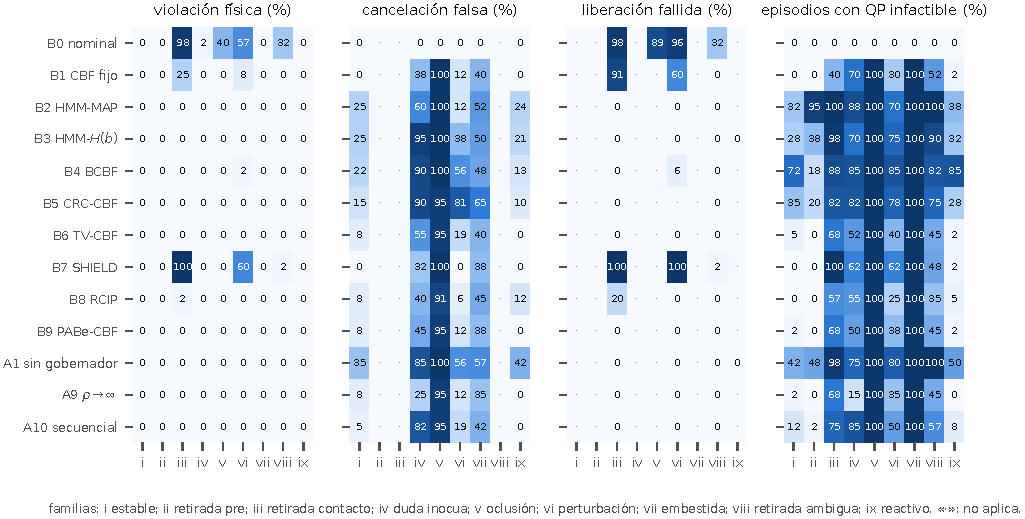
\includegraphics[width=\textwidth]{figures/g1_scenarios.pdf}
\caption{Resultados por escenario (filas: método; columnas: familia). Porcentaje de episodios.}
\label{fig:g1scen}
\end{figure*}

\subsection{Atribución al mecanismo de viabilidad (H1)}
\label{sec:g1:attr}
Para separar el efecto del mecanismo del de la implementación se usaron cuatro controles que comparten
código, señales y umbral, y que sólo difieren en cómo evoluciona $\theta$
(Tabla~\ref{tab:g1attr}, Fig.~\ref{fig:g1attr}):
\begin{enumerate}[label=(\alph*)]
\item \textbf{Equivalencia de implementación.} A9 es el gobernador con $\rho\to\infty$: sólo se aparta de la
referencia $\kappa(\theta^\star-\theta)$ cuando esa referencia es inviable. B6 aplica la misma referencia de
forma exógena. Mientras la viabilidad no restringe, ambos producen la misma trayectoria hasta $3\cdot10^{-5}$\,rad/s.
En 26 de 27 episodios comprobados, la primera divergencia ocurre cuando el QP de B6 es infactible o el gobernador
actúa. El restante es un cambio de conjunto activo del QP provocado por el residuo numérico de $\rho$ finito, con
efecto $\le3\cdot10^{-3}$\,rad/s.
\item \textbf{Mecanismo puro.} Con la misma referencia, A9 reduce los episodios con QP infactible de 55{,}3\,\%
(B6, $\kappa=4$) a 40{,}6\,\%. El gobernador sólo está activo en el 0{,}2\,\% de los ciclos, de modo que la mejora
se debe a la corrección por viabilidad y no a un retoque generalizado de $\theta$.
\item \textbf{Frente a la mejor ley exógena.} Ninguna $\kappa$ iguala al gobernador en ambos ejes
(Fig.~\ref{fig:g1attr}a). Frente a B6$^\ast$, la mejor ley elegida en validación, B9 reduce el jerk en 4{,}6\,m/s$^3$
($p_{\rm Holm}=0{,}004$), pero la diferencia en infactibilidad no es significativa ($-0{,}8$\,pp). Frente a
$\kappa=4$, la reducción es de $-10{,}3$\,pp y $-11{,}5$\,m/s$^3$, y frente a márgenes instantáneos (A1), de $-31{,}9$\,pp.
\item \textbf{Optimización conjunta frente a secuencial.} Hacer avanzar $\theta$ con $u=u_{\rm nom}$ y filtrar $u$
después (A10) aumenta la infactibilidad en 9{,}4\,pp y las cancelaciones falsas en 8{,}6\,pp respecto de B9.
\end{enumerate}
La lectura conjunta es la siguiente. La infactibilidad cae sobre todo por no saltar de margen y por corregir
$\dot\theta$ sólo cuando es inviable (A9). El compromiso de coste de B9 ($\rho$ finito) añade suavidad, pero cuesta
4{,}4\,pp de infactibilidad frente a A9. Una ley exógena bien ajustada recupera la mayor parte del beneficio en
factibilidad. \textbf{H1 se apoya}, con un efecto moderado frente al comparador exógeno más fuerte.

\begin{table*}[!t]
\centering\footnotesize
\caption{Atribución al mecanismo de viabilidad. Todas las variantes comparten código, señales y umbral; sólo cambia cómo evoluciona $\theta$. ``Gob. activo'': \% de ciclos en que el QP conjunto se aparta de la referencia $\kappa(\theta^\star-\theta)$.}
\label{tab:g1attr}
\setlength{\tabcolsep}{3.2pt}
\resizebox{\linewidth}{!}{%
\begin{tabular}{lrrrrrrr}
\toprule
Variante & Infact. \% & Jerk p95 & Viol. \% & Canc. falsa \% & Gob. activo \% & B9$-$X infact. (pp) & B9$-$X jerk \\
\midrule
B6 TV-CBF ($\kappa$=1) & 45{,}8 & 224 & 0{,}0 & 32{,}8 & -- & $-$0{,}8 [$-$2{,}5, 0{,}8] & $-$4{,}6 [$-$6{,}5, $-$2{,}5] \\
B6 TV-CBF ($\kappa$=2) & 48{,}9 & 227 & 0{,}0 & 34{,}0 & -- & $-$3{,}9 [$-$6{,}1, $-$1{,}4] & $-$7{,}7 [$-$10{,}4, $-$5{,}1] \\
B6 TV-CBF ($\kappa$=4) & 55{,}3 & 231 & 0{,}0 & 36{,}0 & -- & $-$10{,}3 [$-$13{,}3, $-$7{,}2] & $-$11{,}5 [$-$14{,}8, $-$8{,}3] \\
B6 TV-CBF ($\kappa$=8) & 62{,}8 & 239 & 0{,}0 & 39{,}6 & -- & $-$17{,}8 [$-$21{,}7, $-$14{,}2] & $-$20{,}0 [$-$26{,}1, $-$14{,}4] \\
B6 TV-CBF ($\kappa$=16) & 69{,}7 & 253 & 0{,}0 & 44{,}4 & -- & $-$24{,}7 [$-$30{,}0, $-$20{,}0] & $-$33{,}3 [$-$43{,}4, $-$24{,}7] \\
B6 TV-CBF ($\kappa$=$\infty$) & 81{,}1 & 296 & 0{,}0 & 44{,}9 & -- & $-$36{,}1 [$-$40{,}3, $-$32{,}2] & $-$76{,}8 [$-$90{,}2, $-$62{,}6] \\
A1 sin gobernador & 76{,}9 & 240 & 0{,}0 & 60{,}3 & -- & $-$31{,}9 [$-$36{,}9, $-$27{,}2] & $-$21{,}0 [$-$25{,}4, $-$16{,}8] \\
A10 secuencial & 54{,}4 & 223 & 0{,}0 & 38{,}4 & 24{,}5 & $-$9{,}4 [$-$13{,}6, $-$5{,}6] & $-$3{,}7 [$-$5{,}7, $-$1{,}8] \\
A9 $\rho\to\infty$ & 40{,}6 & 239 & 0{,}0 & 25{,}4 & 0{,}2 & 4{,}4 [2{,}2, 6{,}9] & $-$19{,}8 [$-$23{,}7, $-$16{,}3] \\
B9 PABe-CBF & 45{,}0 & 219 & 0{,}0 & 29{,}8 & 24{,}9 & -- & -- \\
\bottomrule
\end{tabular}}
\end{table*}


\begin{figure*}[!t]
\centering
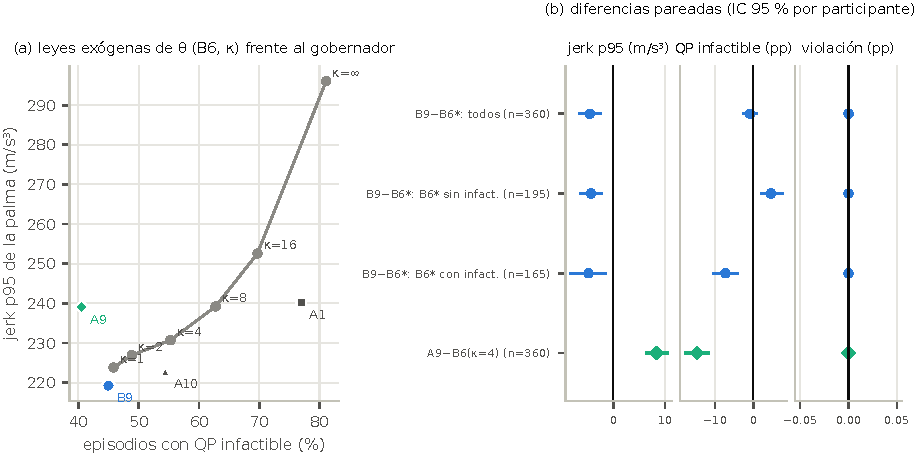
\includegraphics[width=\textwidth]{figures/g1_attribution.pdf}
\caption{(a) Infactibilidad frente a jerk para leyes exógenas de $\theta$ (B6, barrido de $\kappa$) y variantes del
gobernador. (b) Diferencias pareadas: B9$-$B6$^\ast$ en todos los episodios y estratificadas según si B6$^\ast$
perdió la factibilidad; A9$-$B6($\kappa=4$) aísla el mecanismo de viabilidad.}
\label{fig:g1attr}
\end{figure*}

\subsection{Riesgo explícito frente a entropía (H2)}
\label{sec:g1:h2}
B3 cancela 23\,pp más que B9, pero difiere de él en dos cosas: la regla de liberación ($b_W+0{,}4H$) y el uso de
márgenes instantáneos. A1, que usa la regla de B9 con márgenes instantáneos, cancela todavía más (60\,\%). Por eso se
añadió el control A11: idéntico a B9 salvo por la regla de liberación $p_W^+ + 0{,}4H$, con su umbral elegido en
validación. Con la misma sensibilidad (diferencia $-1{,}2$\,pp, n.s.), \textbf{B9 cancela 7{,}6\,pp menos que A11}
(IC [$-$13{,}6, $-$3{,}0], $p_{\rm Holm}=0{,}004$). La diferencia se concentra en la duda inocua (45\,\% frente a 65\,\%)
y en el humano reactivo (0\,\% frente a 10\,\%). En cambio, usar $H$ global en lugar de $E^{\rm exc}$ para los
\emph{márgenes} (A2) no cambia las cancelaciones (+2{,}0\,pp, n.s.). \textbf{H2 se apoya en el G1 para la regla de
liberación}, no para la forma de la incertidumbre que modula los márgenes. Esto corrige la conclusión de la
evaluación planar, donde no se aisló la regla.

\subsubsection*{Experimento controlado: $p_W$ constante, entropía variable}
Durante 0{,}8\,s de contacto con un humano que \emph{no} se retira se impuso a todos los métodos la misma creencia
$b=((1-p)(1-a),(1-p)a,p)$. Con $p$ fijo, $a$ desplaza masa de E a H y aumenta $H$
(Fig.~\ref{fig:g1ctrl}, Tabla~\ref{tab:g1ctrl}). Toda liberación es falsa.
\begin{itemize}
\item \textbf{Métodos que mezclan entropía en la decisión.} B3 pasa del 0\,\% al 100\,\% de liberación al aumentar $H$
con $p=0{,}1$ fijo, y HMM-MAP (B2) libera cuando H se vuelve el estado más probable.
\item \textbf{Métodos que deciden sólo con $p_W$.} B9, B5 y A2 tienen una respuesta invariante a $H$. Su margen
$\theta_d$ sí crece con $E^{\rm exc}$ cuando $p$ es bajo, como prevé el diseño: la incertidumbre pide prudencia,
pero no basta para liberar.
\end{itemize}
Las celdas iso-entropía (Fig.~\ref{fig:g1iso}) reproducen la Proposición~1: con la misma $H$, sólo los métodos que
usan $p_W$ distinguen las creencias con distinto riesgo de retirada.

\subsubsection*{Situaciones en que ambos indicadores discrepan}
En los datos naturales de test, cada tick se clasificó por $H$ (alta/baja) y $b_W$ (baja/media/alta)
(Fig.~\ref{fig:g1disc}). En el cuadrante discrepante ``$H$ alta, $b_W$ baja'' (W real en $\approx$11\,\% de los
ticks), B9 nunca ordena liberar, A11 lo hace en el 2{,}4\,\% de los ticks sin retirada y B3 en el 10{,}7\,\%. En el
cuadrante ambiguo ``$H$ alta, $b_W$ media'' (W real en $\approx$67\,\%), B9 libera en el 78\,\% de los ticks con
retirada y en el 62\,\% de los que no la tienen. A11, B3 y B4 liberan en todos.

\begin{table*}[!t]
\centering\footnotesize
\caption{Contrastes pre-registrados en el G1 (B9 $-$ X; pp o m/s$^3$). Bootstrap pareado remuestreando participantes (4000 réplicas); $p_{Holm}$ sobre los 17 contrastes. B6*: mejor ley exógena elegida en validación.}
\label{tab:g1contrasts}
\setlength{\tabcolsep}{3.2pt}
\resizebox{\linewidth}{!}{%
\begin{tabular}{lllrrrrr}
\toprule
Hip. & Contraste & Métrica & Dif. & IC 95\,\% & $p$ & $p_{Holm}$ & $n$/part. \\
\midrule
H1 & B9 vs B6* & ep. QP infactible & $-$0{,}83 & [$-$2{,}50, 0{,}83] & 0{,}432 & 1{,}000 & 360/20 \\
H1 & B9 vs B6* & jerk p95 & $-$4{,}56 & [$-$6{,}51, $-$2{,}54] & $<$0{,}001 & 0{,}004 & 360/20 \\
H1 & B9 vs B6($\kappa$=4) & ep. QP infactible & $-$10{,}28 & [$-$13{,}33, $-$7{,}22] & $<$0{,}001 & 0{,}004 & 360/20 \\
H1 & B9 vs B6($\kappa$=4) & jerk p95 & $-$11{,}46 & [$-$14{,}79, $-$8{,}25] & $<$0{,}001 & 0{,}004 & 360/20 \\
H1 & B9 vs A1 & ep. QP infactible & $-$31{,}94 & [$-$36{,}94, $-$27{,}22] & $<$0{,}001 & 0{,}004 & 360/20 \\
H1 & B9 vs A1 & violación física & 0{,}00 & [0{,}00, 0{,}00] & 1{,}000 & 1{,}000 & 360/20 \\
H2 & B9 vs B3 & cancelación falsa & $-$23{,}04 & [$-$30{,}27, $-$16{,}15] & $<$0{,}001 & 0{,}004 & 191/20 \\
H2 & B9 vs B3 & sensibilidad & 38{,}89 & [30{,}57, 47{,}20] & $<$0{,}001 & 0{,}004 & 162/20 \\
H2 & B9 vs B5 & cancelación falsa & $-$23{,}74 & [$-$29{,}53, $-$17{,}95] & $<$0{,}001 & 0{,}004 & 198/20 \\
H2 & B9 vs B4 & cancelación falsa & $-$21{,}55 & [$-$28{,}80, $-$14{,}92] & $<$0{,}001 & 0{,}004 & 181/20 \\
H2 & B9 vs B8 & cancelación falsa & $-$2{,}02 & [$-$9{,}55, 4{,}12] & 0{,}664 & 1{,}000 & 198/20 \\
H2 & B9 vs A2 & cancelación falsa & 2{,}02 & [$-$1{,}51, 5{,}70] & 0{,}331 & 1{,}000 & 198/20 \\
H2 & B9 vs A11 & cancelación falsa & $-$7{,}61 & [$-$13{,}57, $-$3{,}02] & $<$0{,}001 & 0{,}004 & 197/20 \\
H2 & B9 vs A11 & sensibilidad & $-$1{,}23 & [$-$4{,}43, 2{,}44] & 0{,}556 & 1{,}000 & 162/20 \\
H3 & B9 vs A5 & violación de eslabón & 0{,}00 & [0{,}00, 0{,}00] & 1{,}000 & 1{,}000 & 360/20 \\
H3 & B9 vs B1 & violación física & $-$3{,}61 & [$-$5{,}56, $-$1{,}94] & $<$0{,}001 & 0{,}004 & 360/20 \\
H3 & B9 vs B1 & liberación fallida & $-$50{,}00 & [$-$75{,}00, $-$25{,}00] & $<$0{,}001 & 0{,}004 & 14/10 \\
\bottomrule
\end{tabular}}
\end{table*}


\begin{figure*}[!t]
\centering
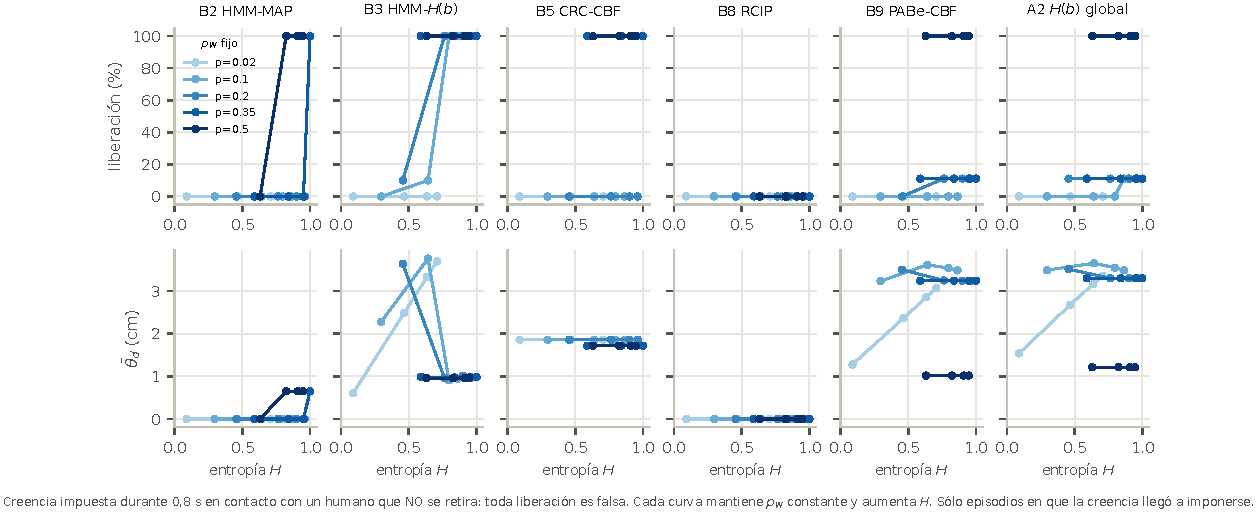
\includegraphics[width=\textwidth]{figures/g1_controlled.pdf}
\caption{Experimento controlado con $p_W$ fijo (color) y entropía creciente. Arriba: probabilidad de liberación
(toda es falsa). Abajo: margen medio $\theta_d$ durante la ventana impuesta.}
\label{fig:g1ctrl}
\end{figure*}

\begin{figure}[!t]
\centering
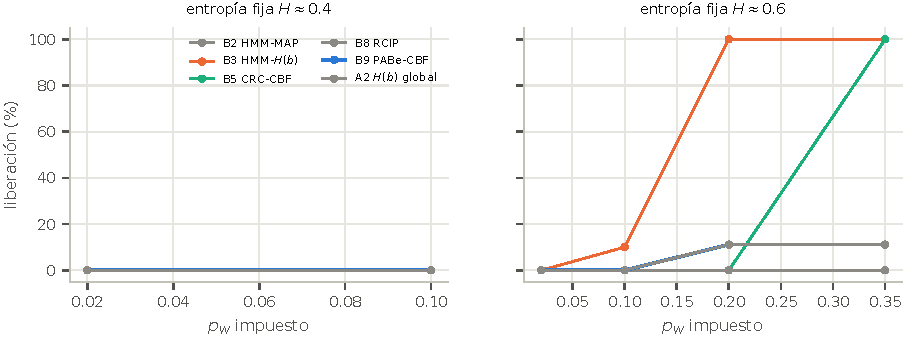
\includegraphics[width=\columnwidth]{figures/g1_isoentropy.pdf}
\caption{Celdas iso-entropía: misma $H$, distinto $p_W$ impuesto.}
\label{fig:g1iso}
\end{figure}

\begin{figure*}[!t]
\centering
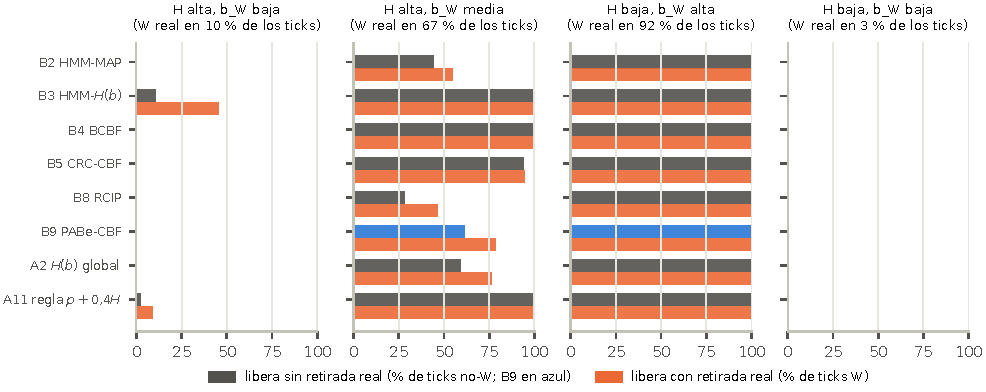
\includegraphics[width=\textwidth]{figures/g1_discrepancy.pdf}
\caption{Decisiones de liberación en los datos de test según el cuadrante ($H$, $b_W$) de la creencia.}
\label{fig:g1disc}
\end{figure*}

\begin{table}[!t]
\centering\footnotesize
\caption{Experimento controlado: probabilidad de liberación (\%) con $p_W$ fijo y entropía creciente ($a$ = fracción de la masa no-W asignada a H). Última columna: cambio del margen medio $\theta_d$ (cm) entre $a=0$ y $a=0{,}5$. El humano no se retira: toda liberación es falsa.}
\label{tab:g1ctrl}
\setlength{\tabcolsep}{3.2pt}
\resizebox{\linewidth}{!}{%
\begin{tabular}{lrrrrrr}
\toprule
Método & $p_W$ & $a$=0 & 0,15 & 0,30 & 0,50 & $\Delta\bar\theta_d$ \\
\midrule
B2 HMM-MAP & 0.1 & 0 & 0 & 0 & 0 & 0{,}0 \\
B2 HMM-MAP & 0.35 & 0 & 0 & 0 & 100 & 0{,}7 \\
B3 HMM-$H(b)$ & 0.1 & 0 & 10 & 100 & 100 & $-$1{,}3 \\
B3 HMM-$H(b)$ & 0.35 & 100 & 100 & 100 & 100 & 0{,}0 \\
B5 CRC-CBF & 0.1 & 0 & 0 & 0 & 0 & 0{,}0 \\
B5 CRC-CBF & 0.35 & 100 & 100 & 100 & 100 & 0{,}0 \\
B8 RCIP & 0.1 & 0 & 0 & 0 & 0 & 0{,}0 \\
B8 RCIP & 0.35 & 0 & 0 & 0 & 0 & 0{,}0 \\
B9 PABe-CBF & 0.1 & 0 & 0 & 0 & 0 & 0{,}3 \\
B9 PABe-CBF & 0.35 & 11 & 11 & 11 & 11 & 0{,}0 \\
A2 $H(b)$ global & 0.1 & 0 & 0 & 0 & 11 & 0{,}0 \\
A2 $H(b)$ global & 0.35 & 11 & 11 & 11 & 11 & 0{,}0 \\
\bottomrule
\end{tabular}}
\end{table}


\subsection{Barreras por eslabón (H3)}
\label{sec:g1:h3}
Ningún método con barreras por eslabón violó la separación de un eslabón no autorizado. Al sustituirlas por una
barrera única (A5) tampoco aparecieron violaciones de eslabón en estos escenarios: el antebrazo del robot rara vez
se acerca al cuerpo humano, salvo en la embestida, donde todos los métodos pierden la factibilidad. A cambio, A5 redujo
las cancelaciones falsas (18{,}7\,\% frente a 29{,}8\,\%) y aumentó el éxito (79{,}8\,\% frente a 64{,}1\,\%).
\textbf{H3 no se apoya en el G1}: en estos escenarios las barreras por eslabón tienen un coste de utilidad sin un
beneficio de seguridad medible. Para justificarlas hacen falta escenarios en que el humano invada la zona
del antebrazo con frecuencia.

\subsection{Sensibilidad a percepción y perturbaciones}
\label{sec:g1:sens}
Seis factores se variaron por separado sobre todas las familias (Fig.~\ref{fig:g1sens}, Tabla~\ref{tab:g1sens}):
\begin{itemize}
\item \textbf{Ruido de posición.} Hasta 4 veces el nominal, de modo que a partir de $\approx$2{,}5 veces se viola la cota $\epsilon_d$.
\item \textbf{Retardo visual adicional.} Hasta 150\,ms.
\item \textbf{Ruido de las observaciones del HMM.} Hasta 3 veces el nominal.
\item \textbf{Empujones de hasta 30\,N sobre el antebrazo.}
\item \textbf{Retardo táctil.} Hasta 0{,}5\,s.
\item \textbf{Amplitud de la embestida.} Hasta 24\,cm.
\end{itemize}
El resultado es claro: la degradación recae en la utilidad y no en la seguridad. B9 no registró violaciones en ningún
nivel; B1 empezó a violar con empujones de 30\,N (3\,\%). En cambio, las cancelaciones falsas de B9 suben del
28\,\% al 82\,\% con 4 veces el ruido de posición y al 100\,\% con 3 veces el ruido de observación: el HMM deja de
distinguir disposición y el filtro se vuelve conservador. Con niveles moderados (2 veces el ruido de posición), B9 se
degrada menos que B3 y B5 (67\,\% frente a 100\,\%).

\begin{figure*}[!t]
\centering
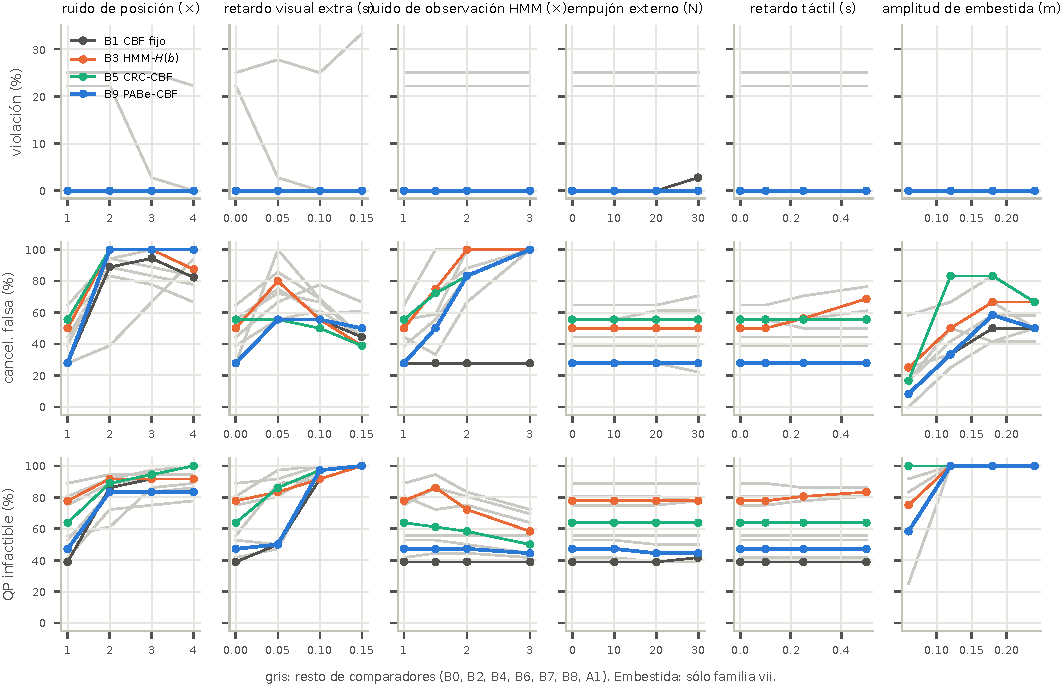
\includegraphics[width=\textwidth]{figures/g1_sensitivity.pdf}
\caption{Sensibilidad: violación física, cancelación falsa y episodios con QP infactible frente a la severidad de cada
factor (36 episodios por nivel y método; 12 en la embestida).}
\label{fig:g1sens}
\end{figure*}

\begin{table*}[!t]
\centering\footnotesize
\caption{Sensibilidad a errores de percepción y perturbaciones: violación\,\% / cancelación falsa\,\% en el nivel más leve y el más severo de cada factor.}
\label{tab:g1sens}
\setlength{\tabcolsep}{3.2pt}
\resizebox{\linewidth}{!}{%
\begin{tabular}{llrrrrrr}
\toprule
Factor & Nivel & B1 & B3 & B5 & B6 & B9 & A1 \\
\midrule
ruido de posición ($\times$) & 1 & 0/28 & 0/50 & 0/56 & 0/39 & 0/28 & 0/65 \\
ruido de posición ($\times$) & 4 & 0/82 & 0/88 & 0/100 & 0/83 & 0/100 & 0/88 \\
retardo visual extra (s) & 0 & 0/28 & 0/50 & 0/56 & 0/39 & 0/28 & 0/65 \\
retardo visual extra (s) & 0.15 & 0/44 & 0/39 & 0/39 & 0/44 & 0/50 & 0/44 \\
ruido de observación HMM ($\times$) & 1 & 0/28 & 0/50 & 0/56 & 0/39 & 0/28 & 0/65 \\
ruido de observación HMM ($\times$) & 3 & 0/28 & 0/100 & 0/100 & 0/100 & 0/100 & 0/100 \\
empujón externo (N) & 0 & 0/28 & 0/50 & 0/56 & 0/39 & 0/28 & 0/65 \\
empujón externo (N) & 30 & 3/28 & 0/50 & 0/56 & 0/39 & 0/28 & 0/71 \\
retardo táctil (s) & 0 & 0/28 & 0/50 & 0/56 & 0/39 & 0/28 & 0/65 \\
retardo táctil (s) & 0.5 & 0/28 & 0/69 & 0/56 & 0/39 & 0/28 & 0/76 \\
amplitud de embestida (m) & 0.06 & 0/8 & 0/25 & 0/17 & 0/17 & 0/8 & 0/58 \\
amplitud de embestida (m) & 0.24 & 0/50 & 0/67 & 0/67 & 0/50 & 0/50 & 0/67 \\
\bottomrule
\end{tabular}}
\end{table*}


\subsection{Comportamiento ante la pérdida temporal de factibilidad}
\label{sec:g1:feas}
En la oclusión y la embestida \emph{todos} los métodos filtrados pierden la factibilidad
(Tabla~\ref{tab:g1feas}, Fig.~\ref{fig:g1feas}). Lo que distingue a los métodos es qué ocurre durante la pérdida:
\begin{itemize}
\item \textbf{B9.} El 45\,\% de sus episodios contiene algún intervalo infactible, con una duración mediana de 105\,ms
(p95 = 390\,ms). Todos los intervalos se recuperaron y ninguno produjo violación física, gracias a la política de
respaldo y a que la pérdida suele deberse a cotas de incertidumbre que se expanden y no a un contacto real.
\item \textbf{SHIELD (B7).} Su margen aprendido no es una cota, y el 34\,\% de sus pérdidas de factibilidad terminan en
violación (de fuerza).
\item \textbf{B1.} El 8\,\% de sus pérdidas termina en violación.
\end{itemize}

\begin{table*}[!t]
\centering\footnotesize
\caption{Comportamiento ante la pérdida temporal de factibilidad (test). Intervalo: desde el primer ciclo infactible hasta que el QP vuelve a ser factible con todas las barreras estimadas $\ge0$.}
\label{tab:g1feas}
\setlength{\tabcolsep}{3.2pt}
\resizebox{\linewidth}{!}{%
\begin{tabular}{lrrrrrr}
\toprule
Método & Ep. con pérdida \% & Intervalos/ep. & Duración mediana (ms) & p95 (ms) & Sin recuperar \% & Violación \% \\
\midrule
B1 CBF fijo & 43{,}9 & 0{,}54 & 120 & 410 & 0{,}0 & 8{,}2 \\
B2 HMM-MAP & 80{,}3 & 1{,}24 & 130 & 642 & 0{,}7 & 0{,}0 \\
B3 HMM-$H(b)$ & 70{,}0 & 0{,}85 & 110 & 454 & 0{,}0 & 0{,}0 \\
B4 BCBF & 79{,}4 & 1{,}25 & 35 & 400 & 0{,}0 & 0{,}3 \\
B5 CRC-CBF & 66{,}7 & 0{,}91 & 125 & 442 & 0{,}0 & 0{,}0 \\
B6 TV-CBF & 45{,}8 & 0{,}53 & 110 & 418 & 0{,}0 & 0{,}0 \\
B7 SHIELD & 52{,}8 & 0{,}57 & 80 & 365 & 0{,}0 & 34{,}2 \\
B8 RCIP & 41{,}9 & 0{,}48 & 110 & 405 & 0{,}0 & 0{,}7 \\
B9 PABe-CBF & 45{,}0 & 0{,}50 & 105 & 390 & 0{,}0 & 0{,}0 \\
A1 sin gobernador & 76{,}9 & 0{,}94 & 110 & 430 & 0{,}0 & 0{,}0 \\
A9 $\rho\to\infty$ & 40{,}6 & 0{,}41 & 100 & 400 & 0{,}0 & 0{,}0 \\
A10 secuencial & 54{,}4 & 0{,}66 & 120 & 410 & 0{,}0 & 0{,}0 \\
\bottomrule
\end{tabular}}
\end{table*}


\begin{figure*}[!t]
\centering
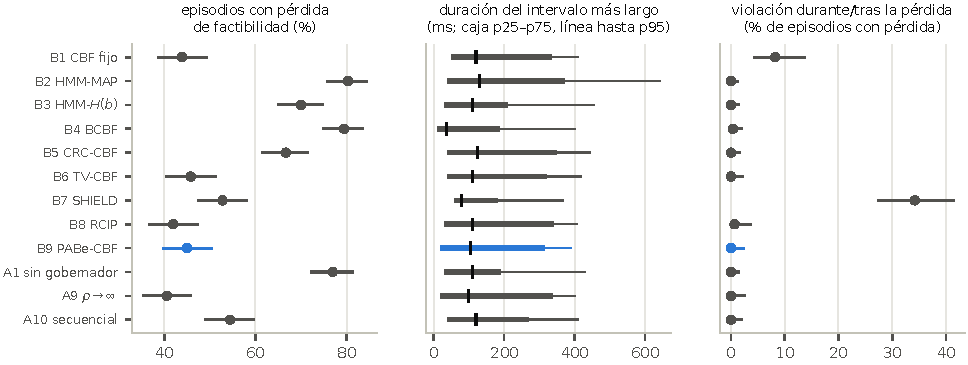
\includegraphics[width=\textwidth]{figures/g1_feasibility.pdf}
\caption{Pérdida temporal de factibilidad: frecuencia, duración del intervalo más largo y violaciones durante o
después de la pérdida.}
\label{fig:g1feas}
\end{figure*}

\subsection{Coste computacional y calibración}
\label{sec:g1:cost}
\begin{itemize}
\item \textbf{Cómputo.} La capa de seguridad de B9 requiere 1{,}27/2{,}10/2{,}22\,ms (p50/p95/p99) por ciclo en Python,
con un máximo de 6{,}0\,ms. El QP conjunto de 9 variables tarda 0{,}21\,ms en la mediana. Ningún ciclo de B9 superó los
150\,ms; en todo el test, sólo 3 de 4{,}4 millones de ciclos lo hicieron, todos de A9 y aislados, atribuibles a la
máquina compartida (Tabla~\ref{tab:g1lat}). A la latencia sensor$\to$actuador modelada se suman 33\,ms de percepción visual y la
dinámica del lazo de par.
\item \textbf{Calibración.} La cota isotónica de $p_W^+$ obtiene un ECE de 0{,}010 frente a 0{,}029 por bins, y un
AUROC de 0{,}931 frente a 0{,}808 (Fig.~\ref{fig:g1rel}).
\item \textbf{Variantes sin beneficio.} El HSMM (A6) no mejora a B9 y la modalidad táctil (A7) no aporta en estos
escenarios, porque la retirada se detecta antes visualmente. En cambio, quitar $p_W^+$ (A3) produce un 3{,}1\,\% de
violaciones y un 31\,\% de liberaciones fallidas, y usar $b_W$ sin calibrar (A4), un 15\,\% de liberaciones fallidas.
\end{itemize}

\begin{table*}[!t]
\centering\footnotesize
\caption{Coste por ciclo de la capa de seguridad en el G1 (ms; Python, 11 procesos concurrentes). La latencia sensor$\to$actuador modelada añade 33\,ms de percepción visual y la dinámica del lazo de par. En total, 3 de 4{,}4 millones de ciclos superaron 150\,ms (todos de A9; picos aislados en una máquina compartida).}
\label{tab:g1lat}
\setlength{\tabcolsep}{3.2pt}
\resizebox{\linewidth}{!}{%
\begin{tabular}{lrrrrrrr}
\toprule
Método & p50 & p95 & p99 & máx & QP p50 & QP p99 & \% $>$150 ms \\
\midrule
B0 nominal & 0{,}361 & 0{,}656 & 0{,}736 & 12{,}8 & 0{,}000 & 0{,}000 & 0{,}00 \\
B1 CBF fijo & 1{,}421 & 2{,}391 & 3{,}267 & 25{,}4 & 0{,}279 & 0{,}551 & 0{,}00 \\
B2 HMM-MAP & 1{,}314 & 2{,}189 & 2{,}474 & 12{,}6 & 0{,}261 & 0{,}462 & 0{,}00 \\
B3 HMM-$H(b)$ & 1{,}252 & 2{,}081 & 2{,}197 & 9{,}9 & 0{,}243 & 0{,}412 & 0{,}00 \\
B4 BCBF & 1{,}577 & 2{,}578 & 2{,}717 & 45{,}2 & 0{,}244 & 0{,}409 & 0{,}00 \\
B5 CRC-CBF & 1{,}296 & 2{,}130 & 2{,}261 & 8{,}9 & 0{,}248 & 0{,}419 & 0{,}00 \\
B6 TV-CBF & 1{,}298 & 2{,}142 & 2{,}290 & 12{,}8 & 0{,}245 & 0{,}421 & 0{,}00 \\
B7 SHIELD & 1{,}438 & 2{,}368 & 2{,}542 & 12{,}2 & 0{,}248 & 0{,}431 & 0{,}00 \\
B8 RCIP & 1{,}712 & 2{,}781 & 2{,}984 & 7{,}7 & 0{,}252 & 0{,}433 & 0{,}00 \\
B9 PABe-CBF & 1{,}267 & 2{,}097 & 2{,}218 & 6{,}0 & 0{,}212 & 0{,}368 & 0{,}00 \\
A6 HSMM & 1{,}287 & 2{,}121 & 2{,}269 & 5{,}8 & 0{,}211 & 0{,}366 & 0{,}00 \\
A9 $\rho\to\infty$ & 1{,}259 & 2{,}076 & 2{,}230 & 1011{,}9 & 0{,}210 & 0{,}364 & 0{,}00 \\
A10 secuencial & 1{,}492 & 2{,}456 & 2{,}612 & 13{,}7 & 0{,}433 & 0{,}741 & 0{,}00 \\
\bottomrule
\end{tabular}}
\end{table*}


\begin{figure}[!t]
\centering
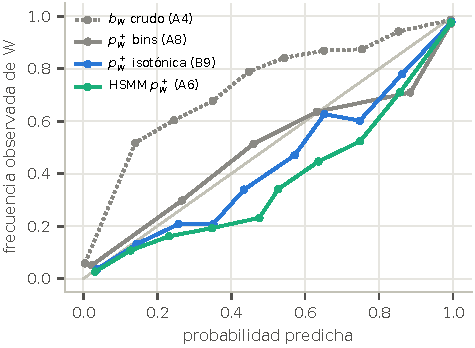
\includegraphics[width=\columnwidth]{figures/g1_reliability.pdf}
\caption{Fiabilidad de la señal de retirada en el G1 (test).}
\label{fig:g1rel}
\end{figure}

\begin{table*}[!t]
\centering\footnotesize
\caption{Resultados por escenario (G1, test).}
\label{tab:g1fam}
\setlength{\tabcolsep}{3.2pt}
\resizebox{\linewidth}{!}{%
\begin{tabular}{llrrrrrr}
\toprule
Familia & Método & Viol. \% & $F$ pico (N) & Canc. falsa \% & Lib. fallida \% & Éxito \% & Infact. \% \\
\midrule
i estable & B0 nominal & 0{,}0 & 9{,}5 & 0{,}0 & -- & 100{,}0 & 0{,}0 \\
 & B1 CBF fijo & 0{,}0 & 10{,}7 & 0{,}0 & -- & 100{,}0 & 0{,}0 \\
 & B2 HMM-MAP & 0{,}0 & 8{,}7 & 25{,}0 & -- & 72{,}5 & 32{,}5 \\
 & B3 HMM-$H(b)$ & 0{,}0 & 8{,}6 & 25{,}0 & -- & 72{,}5 & 27{,}5 \\
 & B4 BCBF & 0{,}0 & 9{,}3 & 22{,}5 & -- & 77{,}5 & 72{,}5 \\
 & B5 CRC-CBF & 0{,}0 & 10{,}5 & 15{,}0 & -- & 82{,}5 & 35{,}0 \\
 & B6 TV-CBF & 0{,}0 & 10{,}7 & 7{,}5 & -- & 92{,}5 & 5{,}0 \\
 & B7 SHIELD & 0{,}0 & 10{,}1 & 0{,}0 & -- & 100{,}0 & 0{,}0 \\
 & B8 RCIP & 0{,}0 & 9{,}2 & 7{,}5 & -- & 82{,}5 & 0{,}0 \\
 & B9 PABe-CBF & 0{,}0 & 9{,}9 & 7{,}5 & -- & 85{,}0 & 2{,}5 \\
\midrule
ii retirada pre & B0 nominal & 0{,}0 & 0{,}0 & -- & -- & 100{,}0 & 0{,}0 \\
 & B1 CBF fijo & 0{,}0 & 0{,}0 & -- & -- & 100{,}0 & 0{,}0 \\
 & B2 HMM-MAP & 0{,}0 & 0{,}0 & -- & -- & 100{,}0 & 95{,}0 \\
 & B3 HMM-$H(b)$ & 0{,}0 & 0{,}0 & -- & -- & 100{,}0 & 37{,}5 \\
 & B4 BCBF & 0{,}0 & 0{,}0 & -- & -- & 100{,}0 & 17{,}5 \\
 & B5 CRC-CBF & 0{,}0 & 0{,}0 & -- & -- & 100{,}0 & 20{,}0 \\
 & B6 TV-CBF & 0{,}0 & 0{,}0 & -- & -- & 100{,}0 & 0{,}0 \\
 & B7 SHIELD & 0{,}0 & 0{,}0 & -- & -- & 100{,}0 & 0{,}0 \\
 & B8 RCIP & 0{,}0 & 0{,}0 & -- & -- & 100{,}0 & 0{,}0 \\
 & B9 PABe-CBF & 0{,}0 & 0{,}0 & -- & -- & 100{,}0 & 0{,}0 \\
\midrule
iii retirada contacto & B0 nominal & 97{,}5 & 33{,}4 & -- & 97{,}5 & -- & 0{,}0 \\
 & B1 CBF fijo & 25{,}0 & 6{,}1 & -- & 90{,}9 & -- & 40{,}0 \\
 & B2 HMM-MAP & 0{,}0 & 0{,}3 & -- & 0{,}0 & -- & 100{,}0 \\
 & B3 HMM-$H(b)$ & 0{,}0 & 1{,}8 & -- & 0{,}0 & -- & 97{,}5 \\
 & B4 BCBF & 0{,}0 & 6{,}7 & -- & 0{,}0 & -- & 87{,}5 \\
 & B5 CRC-CBF & 0{,}0 & 0{,}4 & -- & 0{,}0 & -- & 82{,}5 \\
 & B6 TV-CBF & 0{,}0 & 1{,}5 & -- & 0{,}0 & -- & 67{,}5 \\
 & B7 SHIELD & 100{,}0 & 24{,}6 & -- & 100{,}0 & -- & 100{,}0 \\
 & B8 RCIP & 2{,}5 & 1{,}6 & -- & 20{,}0 & -- & 57{,}5 \\
 & B9 PABe-CBF & 0{,}0 & 1{,}3 & -- & 0{,}0 & -- & 67{,}5 \\
\midrule
iv duda inocua & B0 nominal & 2{,}5 & 9{,}2 & 0{,}0 & -- & 100{,}0 & 0{,}0 \\
 & B1 CBF fijo & 0{,}0 & 5{,}6 & 37{,}5 & -- & 52{,}5 & 70{,}0 \\
 & B2 HMM-MAP & 0{,}0 & 3{,}0 & 60{,}0 & -- & 22{,}5 & 87{,}5 \\
 & B3 HMM-$H(b)$ & 0{,}0 & 1{,}2 & 95{,}0 & -- & 5{,}0 & 70{,}0 \\
 & B4 BCBF & 0{,}0 & 4{,}5 & 90{,}0 & -- & 7{,}5 & 85{,}0 \\
 & B5 CRC-CBF & 0{,}0 & 0{,}0 & 90{,}0 & -- & 0{,}0 & 82{,}5 \\
 & B6 TV-CBF & 0{,}0 & 4{,}4 & 55{,}0 & -- & 40{,}0 & 52{,}5 \\
 & B7 SHIELD & 0{,}0 & 5{,}4 & 32{,}5 & -- & 67{,}5 & 62{,}5 \\
 & B8 RCIP & 0{,}0 & 4{,}8 & 40{,}0 & -- & 42{,}5 & 55{,}0 \\
 & B9 PABe-CBF & 0{,}0 & 4{,}8 & 45{,}0 & -- & 45{,}0 & 50{,}0 \\
\midrule
v oclusión & B0 nominal & 40{,}0 & 21{,}4 & 0{,}0 & 88{,}9 & 100{,}0 & 0{,}0 \\
 & B1 CBF fijo & 0{,}0 & 0{,}0 & 100{,}0 & -- & 0{,}0 & 100{,}0 \\
 & B2 HMM-MAP & 0{,}0 & 0{,}0 & 100{,}0 & -- & 0{,}0 & 100{,}0 \\
 & B3 HMM-$H(b)$ & 0{,}0 & 0{,}0 & 100{,}0 & -- & 0{,}0 & 100{,}0 \\
 & B4 BCBF & 0{,}0 & 0{,}0 & 100{,}0 & -- & 0{,}0 & 100{,}0 \\
 & B5 CRC-CBF & 0{,}0 & 0{,}3 & 95{,}5 & -- & 4{,}5 & 100{,}0 \\
 & B6 TV-CBF & 0{,}0 & 0{,}3 & 95{,}5 & -- & 4{,}5 & 100{,}0 \\
 & B7 SHIELD & 0{,}0 & 0{,}4 & 100{,}0 & -- & 0{,}0 & 100{,}0 \\
 & B8 RCIP & 0{,}0 & 0{,}0 & 90{,}9 & -- & 0{,}0 & 100{,}0 \\
 & B9 PABe-CBF & 0{,}0 & 0{,}3 & 95{,}5 & -- & 4{,}5 & 100{,}0 \\
\midrule
vi perturbación & B0 nominal & 57{,}5 & 23{,}7 & 0{,}0 & 95{,}8 & 100{,}0 & 0{,}0 \\
 & B1 CBF fijo & 7{,}5 & 6{,}4 & 12{,}5 & 60{,}0 & 87{,}5 & 30{,}0 \\
 & B2 HMM-MAP & 0{,}0 & 3{,}4 & 12{,}5 & 0{,}0 & 75{,}0 & 70{,}0 \\
 & B3 HMM-$H(b)$ & 0{,}0 & 4{,}8 & 37{,}5 & 0{,}0 & 56{,}2 & 75{,}0 \\
 & B4 BCBF & 2{,}5 & 9{,}1 & 56{,}2 & 5{,}9 & 43{,}8 & 85{,}0 \\
 & B5 CRC-CBF & 0{,}0 & 0{,}8 & 81{,}2 & -- & 18{,}8 & 77{,}5 \\
 & B6 TV-CBF & 0{,}0 & 4{,}8 & 18{,}8 & 0{,}0 & 81{,}2 & 40{,}0 \\
 & B7 SHIELD & 60{,}0 & 18{,}8 & 0{,}0 & 100{,}0 & 100{,}0 & 62{,}5 \\
 & B8 RCIP & 0{,}0 & 4{,}4 & 6{,}2 & 0{,}0 & 81{,}2 & 25{,}0 \\
 & B9 PABe-CBF & 0{,}0 & 4{,}5 & 12{,}5 & 0{,}0 & 81{,}2 & 37{,}5 \\
\midrule
vii embestida & B0 nominal & 0{,}0 & 8{,}9 & 0{,}0 & -- & 100{,}0 & 0{,}0 \\
 & B1 CBF fijo & 0{,}0 & 6{,}3 & 40{,}0 & -- & 60{,}0 & 100{,}0 \\
 & B2 HMM-MAP & 0{,}0 & 5{,}1 & 52{,}5 & -- & 47{,}5 & 100{,}0 \\
 & B3 HMM-$H(b)$ & 0{,}0 & 5{,}3 & 50{,}0 & -- & 50{,}0 & 100{,}0 \\
 & B4 BCBF & 0{,}0 & 5{,}5 & 47{,}5 & -- & 52{,}5 & 100{,}0 \\
 & B5 CRC-CBF & 0{,}0 & 3{,}9 & 65{,}0 & -- & 35{,}0 & 100{,}0 \\
 & B6 TV-CBF & 0{,}0 & 6{,}4 & 40{,}0 & -- & 60{,}0 & 100{,}0 \\
 & B7 SHIELD & 0{,}0 & 6{,}4 & 37{,}5 & -- & 62{,}5 & 100{,}0 \\
 & B8 RCIP & 0{,}0 & 5{,}2 & 45{,}0 & -- & 50{,}0 & 100{,}0 \\
 & B9 PABe-CBF & 0{,}0 & 6{,}8 & 37{,}5 & -- & 62{,}5 & 100{,}0 \\
\midrule
viii retirada ambigua & B0 nominal & 32{,}5 & 14{,}0 & -- & 32{,}5 & -- & 0{,}0 \\
 & B1 CBF fijo & 0{,}0 & 8{,}1 & -- & 0{,}0 & -- & 52{,}5 \\
 & B2 HMM-MAP & 0{,}0 & 2{,}0 & -- & 0{,}0 & -- & 100{,}0 \\
 & B3 HMM-$H(b)$ & 0{,}0 & 4{,}2 & -- & 0{,}0 & -- & 90{,}0 \\
 & B4 BCBF & 0{,}0 & 7{,}8 & -- & 0{,}0 & -- & 82{,}5 \\
 & B5 CRC-CBF & 0{,}0 & 1{,}7 & -- & 0{,}0 & -- & 75{,}0 \\
 & B6 TV-CBF & 0{,}0 & 2{,}1 & -- & 0{,}0 & -- & 45{,}0 \\
 & B7 SHIELD & 2{,}5 & 14{,}5 & -- & 2{,}5 & -- & 47{,}5 \\
 & B8 RCIP & 0{,}0 & 3{,}1 & -- & 0{,}0 & -- & 35{,}0 \\
 & B9 PABe-CBF & 0{,}0 & 1{,}7 & -- & 0{,}0 & -- & 45{,}0 \\
\midrule
ix reactivo & B0 nominal & 0{,}0 & 9{,}4 & 0{,}0 & -- & 100{,}0 & 0{,}0 \\
 & B1 CBF fijo & 0{,}0 & 10{,}1 & 0{,}0 & -- & 97{,}5 & 2{,}5 \\
 & B2 HMM-MAP & 0{,}0 & 7{,}1 & 24{,}3 & -- & 70{,}3 & 37{,}5 \\
 & B3 HMM-$H(b)$ & 0{,}0 & 8{,}0 & 21{,}2 & 0{,}0 & 78{,}8 & 32{,}5 \\
 & B4 BCBF & 0{,}0 & 5{,}1 & 13{,}0 & -- & 87{,}0 & 85{,}0 \\
 & B5 CRC-CBF & 0{,}0 & 9{,}4 & 10{,}0 & -- & 82{,}5 & 27{,}5 \\
 & B6 TV-CBF & 0{,}0 & 10{,}4 & 0{,}0 & -- & 95{,}0 & 2{,}5 \\
 & B7 SHIELD & 0{,}0 & 10{,}0 & 0{,}0 & -- & 100{,}0 & 2{,}5 \\
 & B8 RCIP & 0{,}0 & 8{,}5 & 12{,}5 & -- & 82{,}5 & 5{,}0 \\
 & B9 PABe-CBF & 0{,}0 & 10{,}1 & 0{,}0 & -- & 90{,}0 & 2{,}5 \\
\bottomrule
\end{tabular}}
\end{table*}


\subsection{Amenazas a la validez}
\label{sec:g1:threats}
\begin{enumerate}[label=(\roman*)]
\item La base está fija y no se modela la locomoción ni el equilibrio.
\item El humano es cinemático, con contacto por resorte. Sólo la familia (ix) reacciona al robot.
\item Las observaciones del HMM son sintéticas.
\item B4, B5, B7 y B8 son adaptaciones. Sus parámetros naturales se ajustaron en validación, pero no se reprodujeron
sus resultados publicados.
\item Las adaptaciones de B4 y B5 y el par adyacente se corrigieron tras una primera ejecución. Las cifras reportadas
proceden de una ejecución completa posterior, con validación y test repetidos.
\item El control A11 se añadió después de ver los resultados para aislar H2, con su propio umbral de validación.
Debe leerse como análisis confirmatorio de un mecanismo, no como contraste pre-registrado.
\item La latencia excluye la percepción real.
\end{enumerate}

\subsection{Síntesis}
\label{sec:g1:summary}
En el G1 simulado, PABe-CBF (B9) no presentó ninguna violación física y ninguna liberación fallida, frente a
un 3--26\,\% de violaciones en los comparadores sin regla de retirada. Sus contribuciones atribuibles son tres:
\begin{itemize}
\item \textbf{Mecanismo de viabilidad.} Con el mismo código, corregir $\dot\theta$ sólo cuando es inviable reduce la
infactibilidad en 15\,pp. Frente a la mejor ley exógena ajustada, la ventaja se limita a la suavidad.
\item \textbf{Regla de liberación basada sólo en $p_W^+$.} Con la misma sensibilidad, cancela 7{,}6\,pp menos que la
misma regla con entropía, y la diferencia se concentra en las situaciones en que entropía y riesgo discrepan.
\item \textbf{Riesgo explícito calibrado.} Es necesario para no fallar las liberaciones.
\end{itemize}
No se encontró beneficio de las barreras por eslabón (H3) ni de la entropía excedente frente a la global en los
márgenes. El rendimiento es frágil ante el ruido de observación del HMM: la seguridad se mantiene, pero la utilidad
colapsa.
